
\documentclass[letterpaper,hide notes,xcolor={table,svgnames},pdftex,10pt]{beamer}
\def\showexamples{t}


%\usepackage[svgnames]{xcolor}

%% Demo talk
%\documentclass[letterpaper,notes=show]{beamer}

\usecolortheme{crane}
\setbeamertemplate{navigation symbols}{}

\usetheme{PlamPittsburgh}
%\usetheme{Frankfurt}

%\usepackage{tipa}

\usepackage{hyperref}
\usepackage{graphicx,xspace}
\usepackage[normalem]{ulem}
\usepackage{multicol}
\usepackage{amsmath,amssymb,amsthm,graphicx,xspace}
\newcommand\SF[1]{$\bigstar$\footnote{SF: #1}}

\usepackage[default]{sourcesanspro}
\usepackage[T1]{fontenc}
\usepackage[scaled]{beramono}
\usepackage{tikzpagenodes}

\newcounter{tmpnumSlide}
\newcounter{tmpnumNote}


% old question code
%\newcommand\question[1]{{$\bigstar$ \small \onlySlide{2}{#1}}}
% \newcommand\nquestion[1]{\ifdefined \presentationonly \textcircled{?} \fi \note{\par{\Large \textbf{?}} #1}}
% \newcommand\nanswer[1]{\note{\par{\Large \textbf{A}} #1}}


 \newcommand\mnote[1]{%
   \addtocounter{tmpnumSlide}{1}
   \ifdefined\showcues {~\tiny\fbox{\arabic{tmpnumSlide}}}\fi
   \note{\setlength{\parskip}{1ex}\addtocounter{tmpnumNote}{1}\textbf{\Large \arabic{tmpnumNote}:} {#1\par}}}

\newcommand\mmnote[1]{\note{\setlength{\parskip}{1ex}#1\par}}

%\newcommand\mnote[2][]{\ifdefined\handoutwithnotes {~\tiny\fbox{#1}}\fi
% \note{\setlength{\parskip}{1ex}\textbf{\Large #1:} #2\par}}

%\newcommand\mnote[2][]{{\tiny\fbox{#1}} \note{\setlength{\parskip}{1ex}\textbf{\Large #1:} #2\par}}

\newcommand\mquestion[2]{{~\color{red}\fbox{?}}\note{\setlength{\parskip}{1ex}\par{\Large \textbf{?}} #1} \note{\setlength{\parskip}{1ex}\par{\Large \textbf{A}} #2\par}\ifdefined \presentationonly \pause \fi}

\newcommand\blackboard[1]{%
\ifdefined   \showblackboard
  {#1}
  \else {\begin{center} \fbox{\colorbox{blue!30}{%
         \begin{minipage}{.95\linewidth}%
           \hspace{\stretch{1}} Some space intentionally left blank; done at the blackboard.%
         \end{minipage}}}\end{center}}%
         \fi%
}



%\newcommand\q{\tikz \node[thick,color=black,shape=circle]{?};}
%\newcommand\q{\ifdefined \presentationonly \textcircled{?} \fi}

\usepackage{listings}
\lstset{basicstyle=\footnotesize\ttfamily,
	breaklines=true,
	aboveskip=15pt,
  	belowskip=15pt,
	frame=lines,
	numbers=left, basicstyle=\scriptsize, numberstyle=\tiny, stepnumber=0, numbersep=2pt
}

\usepackage{siunitx}
\newcommand\sius[1]{\num[group-separator = {,}]{#1}\si{\micro\second}}
\newcommand\sims[1]{\num[group-separator = {,}]{#1}\si{\milli\second}}
\newcommand\sins[1]{\num[group-separator = {,}]{#1}\si{\nano\second}}
\sisetup{group-separator = {,}, group-digits = true}

%% -------------------- tikz --------------------
\usepackage{tikz}
\usetikzlibrary{positioning}
\usetikzlibrary{arrows,backgrounds,automata,decorations.shapes,decorations.pathmorphing,decorations.markings,decorations.text}

\tikzstyle{place}=[circle,draw=blue!50,fill=blue!20,thick, inner sep=0pt,minimum size=6mm]
\tikzstyle{transition}=[rectangle,draw=black!50,fill=black!20,thick, inner sep=0pt,minimum size=4mm]

\tikzstyle{block}=[rectangle,draw=black, thick, inner sep=5pt]
\tikzstyle{bullet}=[circle,draw=black, fill=black, thin, inner sep=2pt]

\tikzstyle{pre}=[<-,shorten <=1pt,>=stealth',semithick]
\tikzstyle{post}=[->,shorten >=1pt,>=stealth',semithick]
\tikzstyle{bi}=[<->,shorten >=1pt,shorten <=1pt, >=stealth',semithick]

\tikzstyle{mut}=[-,>=stealth',semithick]

\tikzstyle{treereset}=[dashed,->, shorten >=1pt,>=stealth',thin]

\usepackage{ifmtarg}
\usepackage{xifthen}
\makeatletter
% new counter to now which frame it is within the sequence
\newcounter{multiframecounter}
% initialize buffer for previously used frame title
\gdef\lastframetitle{\textit{undefined}}
% new environment for a multi-frame
\newenvironment{multiframe}[1][]{%
\ifthenelse{\isempty{#1}}{%
% if no frame title was set via optional parameter,
% only increase sequence counter by 1
\addtocounter{multiframecounter}{1}%
}{%
% new frame title has been provided, thus
% reset sequence counter to 1 and buffer frame title for later use
\setcounter{multiframecounter}{1}%
\gdef\lastframetitle{#1}%
}%
% start conventional frame environment and
% automatically set frame title followed by sequence counter
\begin{frame}%
\frametitle{\lastframetitle~{\normalfont(\arabic{multiframecounter})}}%
}{%
\end{frame}%
}
\makeatother

\makeatletter
\newdimen\tu@tmpa%
\newdimen\ydiffl%
\newdimen\xdiffl%
\newcommand\ydiff[2]{%
    \coordinate (tmpnamea) at (#1);%
    \coordinate (tmpnameb) at (#2);%
    \pgfextracty{\tu@tmpa}{\pgfpointanchor{tmpnamea}{center}}%
    \pgfextracty{\ydiffl}{\pgfpointanchor{tmpnameb}{center}}%
    \advance\ydiffl by -\tu@tmpa%
}
\newcommand\xdiff[2]{%
    \coordinate (tmpnamea) at (#1);%
    \coordinate (tmpnameb) at (#2);%
    \pgfextractx{\tu@tmpa}{\pgfpointanchor{tmpnamea}{center}}%
    \pgfextractx{\xdiffl}{\pgfpointanchor{tmpnameb}{center}}%
    \advance\xdiffl by -\tu@tmpa%
}
\makeatother
\newcommand{\copyrightbox}[3][r]{%
\begin{tikzpicture}%
\node[inner sep=0pt,minimum size=2em](ciimage){#2};
\usefont{OT1}{phv}{n}{n}\fontsize{4}{4}\selectfont
\ydiff{ciimage.south}{ciimage.north}
\xdiff{ciimage.west}{ciimage.east}
\ifthenelse{\equal{#1}{r}}{%
\node[inner sep=0pt,right=1ex of ciimage.south east,anchor=north west,rotate=90]%
{\raggedleft\color{black!50}\parbox{\the\ydiffl}{\raggedright{}#3}};%
}{%
\ifthenelse{\equal{#1}{l}}{%
\node[inner sep=0pt,right=1ex of ciimage.south west,anchor=south west,rotate=90]%
{\raggedleft\color{black!50}\parbox{\the\ydiffl}{\raggedright{}#3}};%
}{%
\node[inner sep=0pt,below=1ex of ciimage.south west,anchor=north west]%
{\raggedleft\color{black!50}\parbox{\the\xdiffl}{\raggedright{}#3}};%
}
}
\end{tikzpicture}
}


%% --------------------

%\usepackage[excludeor]{everyhook}
%\PushPreHook{par}{\setbox0=\lastbox\llap{MUH}}\box0}

%\vspace*{\stretch{1}

%\setbox0=\lastbox \llap{\textbullet\enskip}\box0}

\setlength{\parskip}{\fill}

\newcommand\noskips{\setlength{\parskip}{1ex}}
\newcommand\doskips{\setlength{\parskip}{\fill}}

\newcommand\xx{\par\vspace*{\stretch{1}}\par}
\newcommand\xxs{\par\vspace*{2ex}\par}
\newcommand\tuple[1]{\langle #1 \rangle}
\newcommand\code[1]{{\sf \footnotesize #1}}
\newcommand\ex[1]{\uline{Example:} \ifdefined \presentationonly \pause \fi
  \ifdefined\showexamples#1\xspace\else{\uline{\hspace*{2cm}}}\fi}

\newcommand\ceil[1]{\lceil #1 \rceil}


\AtBeginSection[]
{
   \begin{frame}
       \frametitle{Outline}
       \tableofcontents[currentsection]
   \end{frame}
}



\pgfdeclarelayer{edgelayer}
\pgfdeclarelayer{nodelayer}
\pgfsetlayers{edgelayer,nodelayer,main}

\tikzstyle{none}=[inner sep=0pt]
\tikzstyle{rn}=[circle,fill=Red,draw=Black,line width=0.8 pt]
\tikzstyle{gn}=[circle,fill=Lime,draw=Black,line width=0.8 pt]
\tikzstyle{yn}=[circle,fill=Yellow,draw=Black,line width=0.8 pt]
\tikzstyle{empty}=[circle,fill=White,draw=Black]
\tikzstyle{bw} = [rectangle, draw, fill=blue!20, 
    text width=4em, text centered, rounded corners, minimum height=2em]
    
    \newcommand{\CcNote}[1]{% longname
	This work is licensed under the \textit{Creative Commons #1 3.0 License}.%
}
\newcommand{\CcImageBy}[1]{%
	\includegraphics[scale=#1]{creative_commons/cc_by_30.pdf}%
}
\newcommand{\CcImageSa}[1]{%
	\includegraphics[scale=#1]{creative_commons/cc_sa_30.pdf}%
}
\newcommand{\CcImageNc}[1]{%
	\includegraphics[scale=#1]{creative_commons/cc_nc_30.pdf}%
}
\newcommand{\CcGroupBySa}[2]{% zoom, gap
	\CcImageBy{#1}\hspace*{#2}\CcImageNc{#1}\hspace*{#2}\CcImageSa{#1}%
}
\newcommand{\CcLongnameByNcSa}{Attribution-NonCommercial-ShareAlike}

\newenvironment{changemargin}[1]{% 
  \begin{list}{}{% 
    \setlength{\topsep}{0pt}% 
    \setlength{\leftmargin}{#1}% 
    \setlength{\rightmargin}{1em}
    \setlength{\listparindent}{\parindent}% 
    \setlength{\itemindent}{\parindent}% 
    \setlength{\parsep}{\parskip}% 
  }% 
  \item[]}{\end{list}} 



\title{Lecture 4 --- Cache Coherency }

\author{Jeff Zarnett \\ \small \texttt{jzarnett@uwaterloo.ca}}
\institute{Department of Electrical and Computer Engineering \\
  University of Waterloo}
\date{\today}


\begin{document}

\begin{frame}
  \titlepage

 \end{frame}

%%%%%%%%%%%%%%%%%%%%%%%%%%%%%%%%%%%%%%%%%%%%%%%%%%%%%%%%%%%%%%%%%%%%%%%%%%%%%%%%
\begin{frame}
  \frametitle{Introduction}

  \begin{center}
    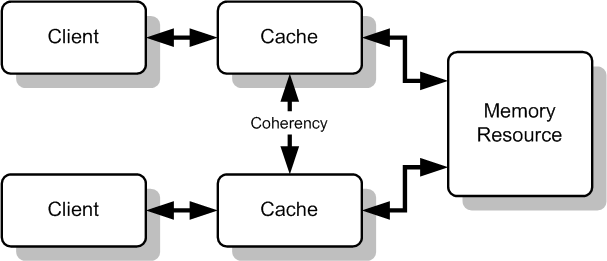
\includegraphics[scale=0.7]{images/coherency}

    Image courtesy of Wikipedia.
  \end{center}
\Large
Each CPU has its own cache: coordination is needed!
  
  {\bf Coherency:}
  \begin{itemize}
    \item Values in all caches are consistent;
    \item System behaves as if all CPUs are using shared memory.
  \end{itemize}
  
\end{frame}
%%%%%%%%%%%%%%%%%%%%%%%%%%%%%%%%%%%%%%%%%%%%%%%%%%%%%%%%%%%%%%%%%%%%%%%%%%%%%%%%

%%%%%%%%%%%%%%%%%%%%%%%%%%%%%%%%%%%%%%%%%%%%%%%%%%%%%%%%%%%%%%%%%%%%%%%%%%%%%%%%
\begin{frame}
  \frametitle{Cache Coherence Example}
\Large

  
  Initially in main memory: {\tt x = 7}.

  \begin{enumerate}
    \item {\tt CPU1} reads x, puts the value in its cache.
    \item {\tt CPU3} reads x, puts the value in its cache.
    \item {\tt CPU3} modifies {\tt x := 42}
    \item {\tt CPU1} reads x \ldots ~from its cache?
    \item {\tt CPU2} reads x. Which value does it get?
  \end{enumerate}
  ~\\

  Unless we do something, {\tt CPU1} is going to read invalid data.
  
\end{frame}
%%%%%%%%%%%%%%%%%%%%%%%%%%%%%%%%%%%%%%%%%%%%%%%%%%%%%%%%%%%%%%%%%%%%%%%%%%%%%%%%



\begin{frame}
\frametitle{Planes and Trains}
\begin{center}
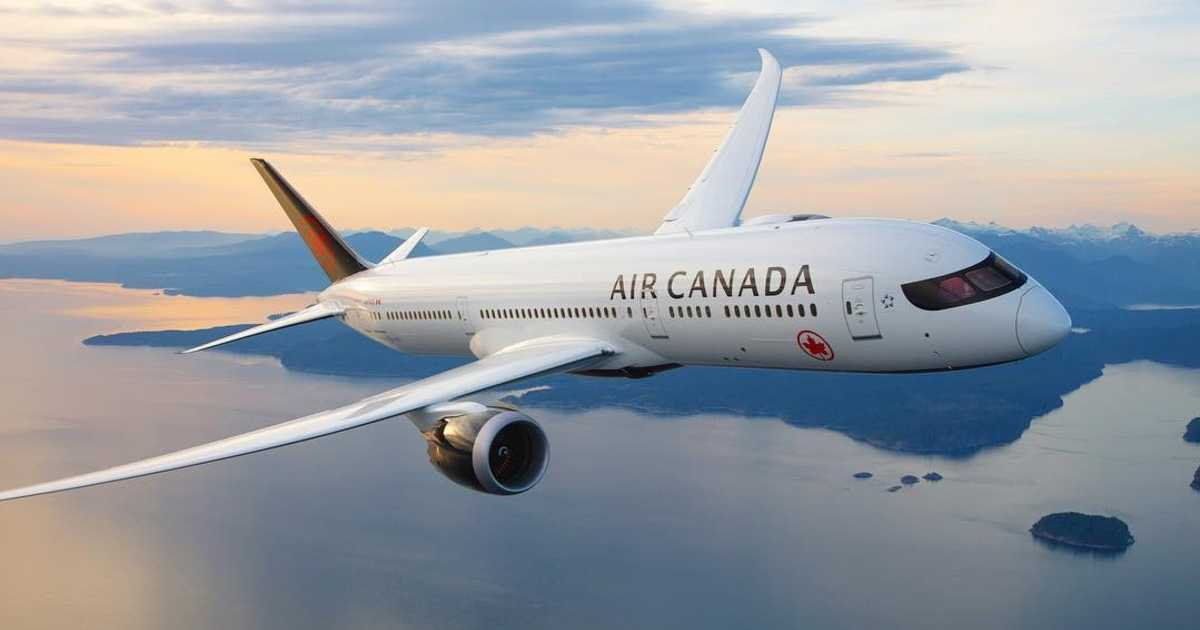
\includegraphics[width=0.5\textwidth]{images/aircanada.jpg}
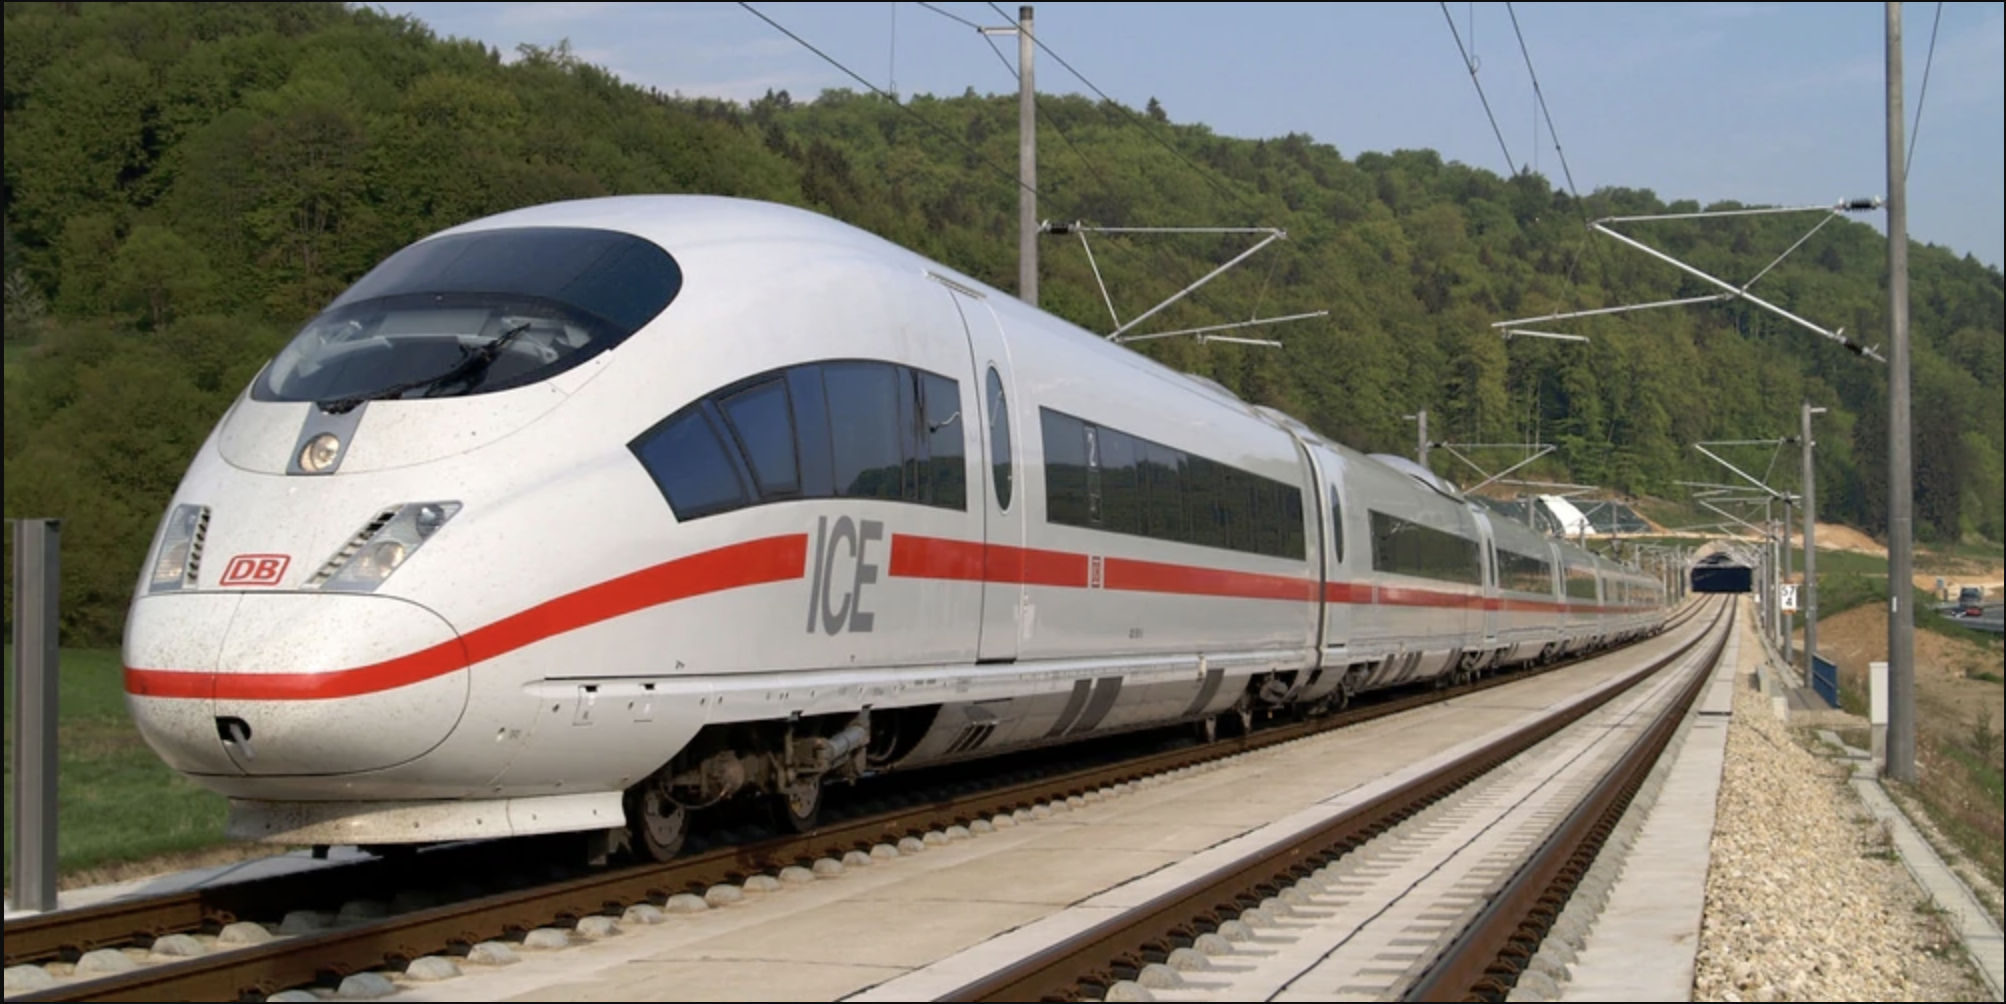
\includegraphics[width=0.5\textwidth]{images/deutschebahn.png}
\end{center}
\end{frame}



\begin{frame}
\frametitle{Snoopy Caches}
\Large

The simplest way to ``do something''
is to use Snoopy caches. 

No, not this kind of Snoopy (sadly):

\begin{center}
	
\includegraphics[width=0.4\textwidth]{images/peanuts-snoopy1.jpg}
\end{center}



\end{frame}

%%%%%%%%%%%%%%%%%%%%%%%%%%%%%%%%%%%%%%%%%%%%%%%%%%%%%%%%%%%%%%%%%%%%%%%%%%%%%%%%
\begin{frame}
  \frametitle{High-Level Explanation of Snoopy Caches}
\Large

  Snoopy: the caches are spying on each other.
  
  \begin{itemize}
    \item Each CPU is connected to a simple bus.
    \item Each CPU ``snoops'' to observe if a memory location is read or written
      by another CPU.
    \item We need a cache controller for every CPU.
  \end{itemize}
  ~\\
  {\bf What happens?}

  \begin{itemize}
    \item Each CPU reads the bus to see if any memory operation is relevant. If
      it is, the controller takes appropriate action.
  \end{itemize}
  
\end{frame}
%%%%%%%%%%%%%%%%%%%%%%%%%%%%%%%%%%%%%%%%%%%%%%%%%%%%%%%%%%%%%%%%%%%%%%%%%%%%%%%%

\begin{frame}
\frametitle{A Distributed Approach}

\Large

This is a distributed approach; \\
no centralized state maintained. 

Each cache with a copy of data from a block of physical memory knows whether it is shared or not. 

Whenever a CPU issues a memory write, the other CPUs are watching (snooping around) to observe if that memory location is in their cache. 

If it is, then the CPU will need to take action.

\end{frame}


\begin{frame}
\frametitle{We Need Some Action!}
\Large

What does action mean?

The Air Canada action was \alert{update}.

The Deutsche Bahn action was \alert{invalidate}.

\end{frame}


%%%%%%%%%%%%%%%%%%%%%%%%%%%%%%%%%%%%%%%%%%%%%%%%%%%%%%%%%%%%%%%%%%%%%%%%%%%%%%%%
\begin{frame}
  \frametitle{Write-Through Cache}
\Large
  
Simplest type of cache coherence:
  \begin{itemize}
    \item All cache writes are done to main memory.
    \item All cache writes also appear on the bus.
    \item If another CPU snoops and sees it has the same location in
      its cache, it will either {\it invalidate} or {\it update} the
      data.
\end{itemize}
~\\

    For write-through caches: normally, when you write to an invalidated
    location, you bypass the cache and go directly to memory (aka {\bf
      write no-allocate}).

  
\end{frame}
%%%%%%%%%%%%%%%%%%%%%%%%%%%%%%%%%%%%%%%%%%%%%%%%%%%%%%%%%%%%%%%%%%%%%%%%%%%%%%%%


\begin{frame}
\frametitle{The Daaaaaaaaaleks!}
\Large

Our chosen approach:

\begin{center}

\includegraphics[width=0.6\textwidth]{images/dalek-invalidate.jpg}
\end{center}

\end{frame}



\begin{frame}
\frametitle{In-val-i-daaaaaate!}
\large

Invalidation is the most common protocol:

\qquad the data in the cache of other CPUs is not updated, \\
\qquad just noted as being out of date (invalid).  

Normally, when you write to an invalidated location, you bypass the cache and go directly to memory.\\
\qquad \qquad (aka {\bf write no-allocate}). 

If we want to do a read and there's a miss, \\
we can poke around in other caches \\
to see who has the most recent cached version. 

This is a bit like going into a room and yelling ``Does anybody have block...?'', in some sort of multicast version of the card game ``Go Fish''. 

Regardless, the most recent value appears in memory, always.


\end{frame}



\begin{frame}
\frametitle{Let's Yell}
\Large

There are also write broadcast protocols, \\
in which case all versions in all caches get updated when there is a write to a shared block. 

But it uses lots of bandwidth and is not necessarily a good idea. 

It does, however prevent the costly cache miss that follows an invalidate. 

Sadly, as we are mere users and not hardware architects, we don't get to decide; we just have to live with whichever one is on the hardware we get. Bummer.


\end{frame}

%%%%%%%%%%%%%%%%%%%%%%%%%%%%%%%%%%%%%%%%%%%%%%%%%%%%%%%%%%%%%%%%%%%%%%%%%%%%%%%%
\begin{frame}
  \frametitle{Write-Through Protocol}
\Large
  
  \begin{itemize}
    \item Two states, {\bf valid} and {\bf invalid}, for each memory location.
    \item Events are either from a processor ({\bf Pr}) or the {\bf Bus}.
  \end{itemize}
  \vfill
  \begin{center}
    \begin{tabular}{llll}
      {\bf State} & {\bf Observed} & {\bf Generated} & {\bf Next State}\\
      Valid   & PrRd  &       & Valid\\
      Valid   & PrWr  & BusWr & Valid\\
      Valid   & BusWr &       & Invalid\\
      Invalid & PrWr  & BusWr & Valid\\
      Invalid & PrRd  & BusRd & Valid\\
    \end{tabular}
  \end{center}
  
\end{frame}
%%%%%%%%%%%%%%%%%%%%%%%%%%%%%%%%%%%%%%%%%%%%%%%%%%%%%%%%%%%%%%%%%%%%%%%%%%%%%%%%

%%%%%%%%%%%%%%%%%%%%%%%%%%%%%%%%%%%%%%%%%%%%%%%%%%%%%%%%%%%%%%%%%%%%%%%%%%%%%%%%
\begin{frame}
  \frametitle{Write-Through Protocol Example}
\large
  

  \begin{itemize}
    \item For simplicity (this isn't an architecture course), assume all cache
      reads/writes are atomic.
  \end{itemize}
  \vfill
  {\bf Using the same example as before:}

  Initially in main memory: {\tt x = 7}.

  \begin{enumerate}
    \item {\tt CPU1} reads x, puts the value in its cache. \structure{(valid)}
    \item {\tt CPU3} reads x, puts the value in its cache. \structure{(valid)}
    \item {\tt CPU3} modifies {\tt x := 42}. \structure{(write to memory)}
      \begin{itemize}
        \item \structure{{\tt CPU1} snoops and marks data as invalid.}
      \end{itemize}
    \item {\tt CPU1} reads x, \structure{from main memory. (valid)}
    \item {\tt CPU2} reads x, \structure{from main memory. (valid)}
  \end{enumerate}
  
\end{frame}
%%%%%%%%%%%%%%%%%%%%%%%%%%%%%%%%%%%%%%%%%%%%%%%%%%%%%%%%%%%%%%%%%%%%%%%%%%%%%%%%

%%%%%%%%%%%%%%%%%%%%%%%%%%%%%%%%%%%%%%%%%%%%%%%%%%%%%%%%%%%%%%%%%%%%%%%%%%%%%%%%
\begin{frame}
  \frametitle{Write-Back Cache}
\Large

     What if, in our example, {\tt CPU3} writes to {\tt x} \\ 3 times?
    \begin{itemize}

    \item Main goal: delay the write to memory as long as possible.\\[1em]
    \item At minimum, we have to add a ``dirty'' bit:\\
     \quad Indicates our data has not yet been written to memory.
  \end{itemize}
  

\end{frame}
%%%%%%%%%%%%%%%%%%%%%%%%%%%%%%%%%%%%%%%%%%%%%%%%%%%%%%%%%%%%%%%%%%%%%%%%%%%%%%%%

%%%%%%%%%%%%%%%%%%%%%%%%%%%%%%%%%%%%%%%%%%%%%%%%%%%%%%%%%%%%%%%%%%%%%%%%%%%%%%%%
\begin{frame}
  \frametitle{Write-Back Implementation}
\large
  
     The simplest type of write-back protocol (MSI), with 3 states:
      \begin{itemize}
        \item {\bf Modified}---only this cache has a valid copy; \\
          \quad main memory is {\bf out-of-date}.
        \item {\bf Shared}---location is unmodified, \\
          \quad up-to-date with main
          memory; \\
          \quad may be present in other caches (also up-to-date).
        \item {\bf Invalid}---same as before.
      \end{itemize}~\\
      
     Initial state, upon first read, is ``shared''.\\[1em]

     Implementation will only write the data to memory \\if another
        processor requests it.\\[1em]

     During write-back, a processor \\
     may read the data from the bus.
  
\end{frame}
%%%%%%%%%%%%%%%%%%%%%%%%%%%%%%%%%%%%%%%%%%%%%%%%%%%%%%%%%%%%%%%%%%%%%%%%%%%%%%%%

%%%%%%%%%%%%%%%%%%%%%%%%%%%%%%%%%%%%%%%%%%%%%%%%%%%%%%%%%%%%%%%%%%%%%%%%%%%%%%%%
\begin{frame}
  \frametitle{MSI Protocol}
\large
  
  \begin{itemize}
    \item Bus write-back (or flush) is {\bf BusWB}.
    \item Exclusive read on the bus is {\bf BusRdX}.
  \end{itemize}~\\

  \begin{center}
    \begin{tabular}{llll}
      {\bf State} & {\bf Observed} & {\bf Generated} & {\bf Next State}\\
      Modified   & PrRd   &        & Modified\\
      Modified   & PrWr   &        & Modified\\
      Modified   & BusRd  & BusWB  & Shared\\
      Modified   & BusRdX & BusWB  & Invalid\\
      Shared     & PrRd   &        & Shared\\
      Shared     & BusRd  &        & Shared\\
      Shared     & BusRdX &        & Invalid\\
      Shared     & PrWr   & BusRdX & Modified\\
      Invalid    & PrRd   & BusRd  & Shared\\
      Invalid    & PrWr   & BusRdX & Modified\\
    \end{tabular}
  \end{center}
  
\end{frame}
%%%%%%%%%%%%%%%%%%%%%%%%%%%%%%%%%%%%%%%%%%%%%%%%%%%%%%%%%%%%%%%%%%%%%%%%%%%%%%%%

%%%%%%%%%%%%%%%%%%%%%%%%%%%%%%%%%%%%%%%%%%%%%%%%%%%%%%%%%%%%%%%%%%%%%%%%%%%%%%%%
\begin{frame}
  \frametitle{MSI Example}

\large  

  {\bf Using the same example as before:}

  Initially in main memory: {\tt x = 7}.

  \begin{enumerate}
    \item {\tt CPU1} reads x from memory. \structure{(BusRd, shared)}
    \item {\tt CPU3} reads x from memory. \structure{(BusRd, shared)}
    \item {\tt CPU3} modifies {\tt x = 42}:
      \begin{itemize}
        \item \structure{Generates a BusRdX.}
        \item \structure{{\tt CPU1} snoops and invalidates x.}
        \item \structure{{\tt CPU3} changes {\tt x}'s state to modified.}
      \end{itemize}
    \item {\tt CPU1} reads x:
      \begin{itemize}
        \item \structure{Generates a BusRd.}
        \item \structure{{\tt CPU3} writes back the data and sets x to shared.}
        \item \structure{{\tt CPU1} reads the new value from the bus as shared.}
      \end{itemize}
    \item {\tt CPU2} reads x from memory. \structure{(BusRd, shared)}
  \end{enumerate}
  
\end{frame}
%%%%%%%%%%%%%%%%%%%%%%%%%%%%%%%%%%%%%%%%%%%%%%%%%%%%%%%%%%%%%%%%%%%%%%%%%%%%%%%%

%%%%%%%%%%%%%%%%%%%%%%%%%%%%%%%%%%%%%%%%%%%%%%%%%%%%%%%%%%%%%%%%%%%%%%%%%%%%%%%%
\begin{frame}
  \frametitle{An Extension to MSI: MESI}
\large
  
    The most common protocol for cache coherence is MESI.\\[1em]
    Adds another state:
      \begin{itemize}
        \item {\bf Modified}---only this cache has a valid copy; \\
\qquad main memory is {\bf out-of-date}.
        \item {\bf Exclusive}---only this cache has a valid copy; \\
\qquad main memory is {\bf up-to-date}.
        \item {\bf Shared}---same as before.
        \item {\bf Invalid}---same as before.
      \end{itemize}
~\\

    MESI allows a processor to modify data exclusive to it, \\without
      having to communicate with the bus.\\
    MESI is \structure{safe}: in E state, no other processor has the
      data.
  
\end{frame}
%%%%%%%%%%%%%%%%%%%%%%%%%%%%%%%%%%%%%%%%%%%%%%%%%%%%%%%%%%%%%%%%%%%%%%%%%%%%%%%%

%%%%%%%%%%%%%%%%%%%%%%%%%%%%%%%%%%%%%%%%%%%%%%%%%%%%%%%%%%%%%%%%%%%%%%%%%%%%%%%%
\begin{frame}
  \frametitle{Even More States!}
\large
  
    MESIF (used in latest i7 processors):
      \begin{itemize}
        \item {\bf Forward}---basically a shared state; but, current
          cache is the only one that will respond to a request to
          transfer the data.
      \end{itemize}~\\[1em]

    Hence: a processor requesting data that is already shared or exclusive will
      only get one response transferring the data.\\[1em]
    Permits more efficient usage of the bus.
  
\end{frame}
%%%%%%%%%%%%%%%%%%%%%%%%%%%%%%%%%%%%%%%%%%%%%%%%%%%%%%%%%%%%%%%%%%%%%%%%%%%%%%%%



\begin{frame}[fragile]
\frametitle{False Sharing}
\Large
False sharing: program has two unrelated data elements that are mapped to the same cache line/location.

\begin{lstlisting}[language=C]
char a[10];
char b[10];
\end{lstlisting}

They don't overlap but are located next to each other in memory.

\end{frame}


\begin{frame}
\frametitle{False Sharing}
\Large
Solution: Heap allocation? Maybe\ldots

Make both arrays bigger, \\
wasting some space\ldots?
\end{frame}


\begin{frame}
\frametitle{False Sharing}

\begin{center}
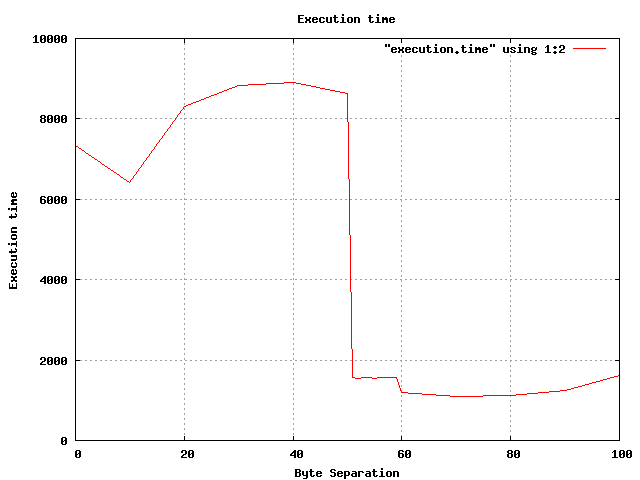
\includegraphics[width=0.6\textwidth]{images/falsesharing.png}
\end{center}
\Large

Is wasting a little space worth it? Yes!
\end{frame}

%%%%%%%%%%%%%%%%%%%%%%%%%%%%%%%%%%%%%%%%%%%%%%%%%%%%%%%%%%%%%%%%%%%%%%%%%%%%%%%%
\begin{frame}[fragile]
  \frametitle{He's a little volatile...}
\Large
  
  {\bf I read that {\tt volatile} variables aren't stored in registers,
     should I worry?}
  \vspace{6.2em}
  \pause

  \begin{center}
    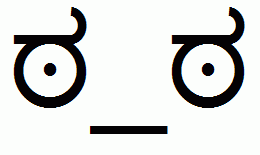
\includegraphics[scale=0.3]{images/disapproval}    
  \end{center}
  
\end{frame}
%%%%%%%%%%%%%%%%%%%%%%%%%%%%%%%%%%%%%%%%%%%%%%%%%%%%%%%%%%%%%%%%%%%%%%%%%%%%%%%%


%%%%%%%%%%%%%%%%%%%%%%%%%%%%%%%%%%%%%%%%%%%%%%%%%%%%%%%%%%%%%%%%%%%%%%%%%%%%%%%%
\begin{frame}[fragile]
  \frametitle{He's a little volatile...}

  
  {\bf I read that {\tt volatile} variables aren't stored in registers,
     should I worry?}

    {\tt volatile} in C was only designed to:
      \begin{itemize}
        \item Allow access to memory mapped devices.
        \item Allow uses of variables between {\tt setjmp} and {\tt longjmp}.
        \item Allow uses of {\tt sig\_atomic\_t} variables in signal handlers.
      \end{itemize}~\\[1em]
    Remember, things can also be reordered by the compiler,
      {\tt volatile} doesn't prevent this.\\[1em]
    Also, it's likely your variables could be in registers the majority
      of the time, except in critical areas.
  
\end{frame}
%%%%%%%%%%%%%%%%%%%%%%%%%%%%%%%%%%%%%%%%%%%%%%%%%%%%%%%%%%%%%%%%%%%%%%%%%%%%%%%%

%%%%%%%%%%%%%%%%%%%%%%%%%%%%%%%%%%%%%%%%%%%%%%%%%%%%%%%%%%%%%%%%%%%%%%%%%%%%%%%%
\begin{frame}
  \frametitle{Cache Coherency Summary}

  
We saw the basics of cache coherence (good to know, but more of an architecture
      thing).
      
There are many other protocols for cache coherence, each with their own
      trade-offs.\\[1em]


  
\end{frame}
%%%%%%%%%%%%%%%%%%%%%%%%%%%%%%%%%%%%%%%%%%%%%%%%%%%%%%%%%%%%%%%%%%%%%%%%%%%%%%%%

\end{document}

